\documentclass[12pt]{article}
\usepackage[utf8]{inputenc}
\usepackage{graphicx} % Allows you to insert figures
\usepackage{amsmath} % Allows you to do equations
\usepackage{fancyhdr} % Formats the header
\usepackage{geometry} % Formats the paper size, orientation, and margins
\linespread{1.25} % about 1.5 spacing in Word
\setlength{\parindent}{0pt} % no paragraph indents
\setlength{\parskip}{1em} % paragraphs separated by one line
\usepackage[format=plain,
            font=it]{caption} % Italicizes figure captions
\usepackage[english]{babel}
\usepackage{csquotes}
\renewcommand{\headrulewidth}{0pt}
\geometry{letterpaper, portrait, margin=1in}
\setlength{\headheight}{14.49998pt}
\geometry{a4paper, left=20mm, right=20mm, top=35mm, bottom=20mm}

\newcommand\titleofdoc{\LARGE{\textbf{Assignment-7: Circuit analysis using SymPy}}}
\newcommand\GroupName{EE20B136}

\begin{document}
\begin{titlepage}
   \begin{center}
        \vspace*{4cm} % Adjust spacings to ensure the title page is generally filled with text

        \Huge{\titleofdoc} 

        \vspace{3 cm}
        \Large{Syam SriBalaji T}
       
        \vspace{0.25cm}
        \large{EE20B136}
       
        \vspace{3 cm}
        \Large{April 01, 2022}
        
        \vspace{0.25 cm}
        \Large{EE2703 :Jan-May 2022}
       

       \vfill
    \end{center}
\end{titlepage}

\setcounter{page}{2}
\pagestyle{fancy}
\fancyhf{}
\rhead{\thepage}

\section*{Magnitude response $|H(j\omega)|$ vs $\omega$ of Low pass filter:}

Here is the plot of $|H(j\omega)|$ vs $\omega$ of LPF,\\
We can clearly notice that this filter only allows waves with low frequency and neglects waves with high frequency.

\begin{figure}[h!]
\centering
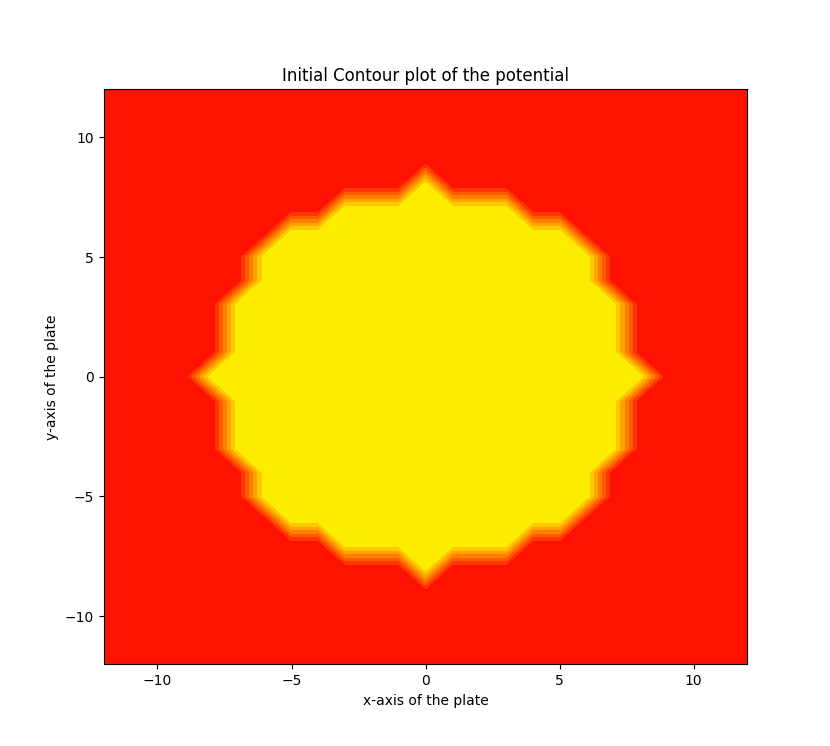
\includegraphics[height=12cm]{Figure_1.png}
\end{figure}

\newpage
\section*{Output responses of Mixed frequency sinusoidal inputs:}

We input a range of frequencies in the below present Input voltage formula, 
\begin{equation*}
V_{i}=(sin(2000\pi t)+cos(2000000\pi t))\times u_{o}(t)
\end{equation*}
And we get a range of input plots 'blue' and while the Output voltage value obtained from 'lsim' function from scipy.signal is also plotted 'red'. It is sinusoidal.\\


\begin{figure}[h!]
\centering
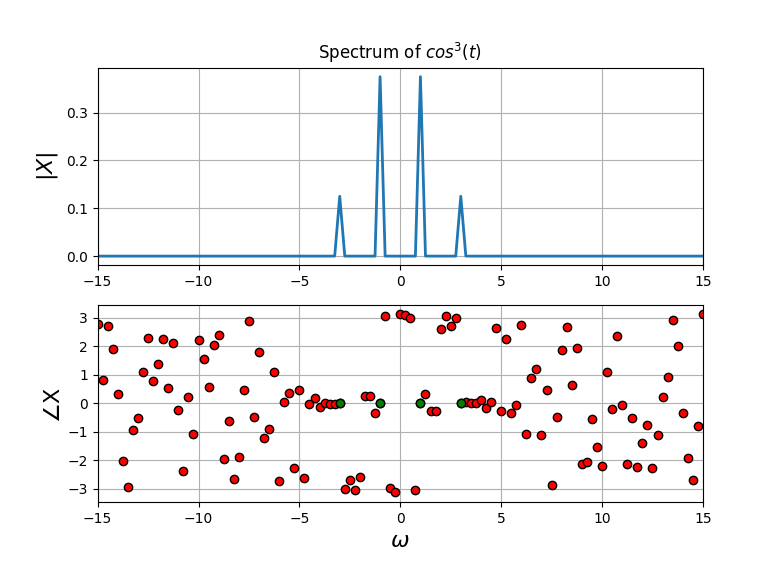
\includegraphics[height=12cm]{Figure_2.png}
\end{figure}

\newpage
\section*{Step response of the Low pass filter:}

Step response of LPF is obtained from 'step' function from scipy.signal\\\\
Here we can notice that the Output voltage is zero in the beginning, and then increases drastically and remains constant over rest of the time.

\begin{figure}[h!]
\centering
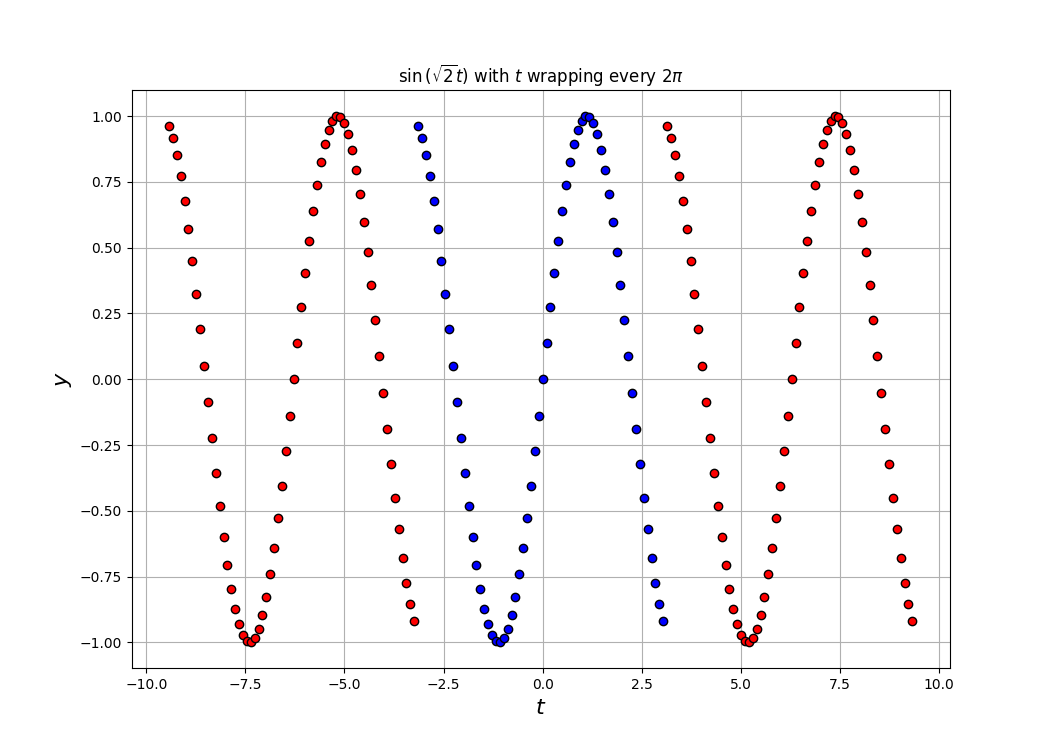
\includegraphics[height=11cm]{Figure_3.png}
\label{fig:exemplo}
\end{figure}


\newpage
\section*{Magnitude response $|H(j\omega)|$ vs $\omega$ of High pass filter:}

Here is the plot of $|H(j\omega)|$ vs $\omega$ of HPF,\\
We can clearly notice that this filter only allows waves with high frequency and neglects waves with low frequency.

\begin{figure}[h!]
\centering
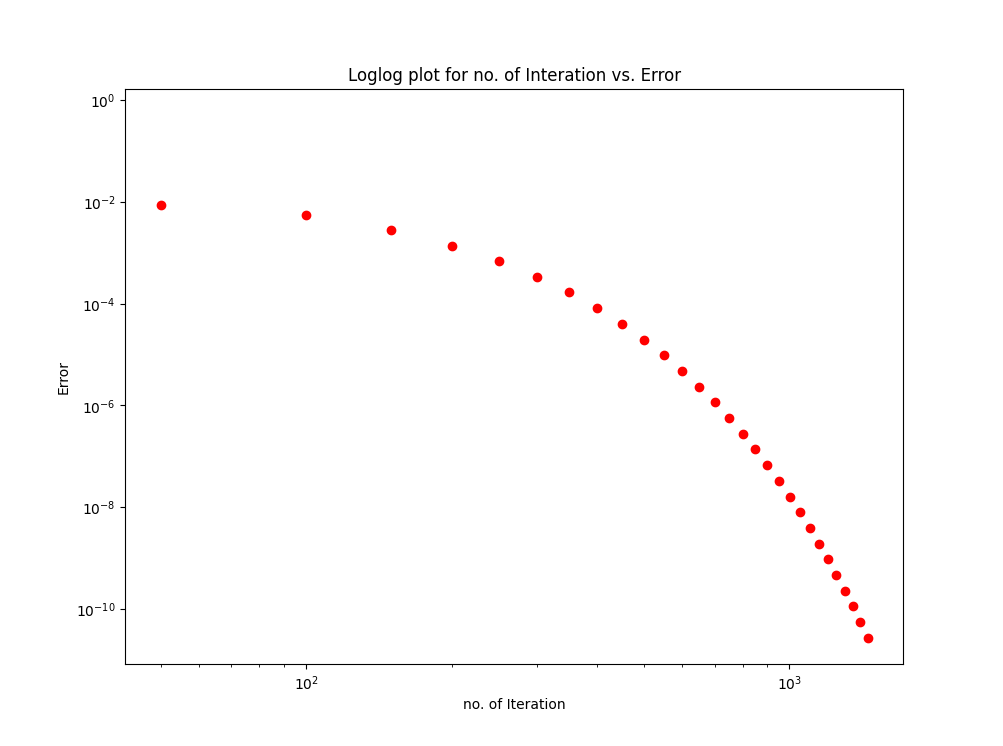
\includegraphics[height=12cm]{Figure_4.png}
\label{fig:exemplo}
\end{figure}

\newpage
\section*{Response of Damped sinusoidal with input of $1$ Hz in HPF:}

Here is the Input and Output voltage plots for Damped sinusoidal inputs with 1 Hz frequency.\\\\
We can clearly notice the damping in Input voltage while the Output voltage almost remains zero over the whole time interval.

\begin{figure}[h!]
\centering
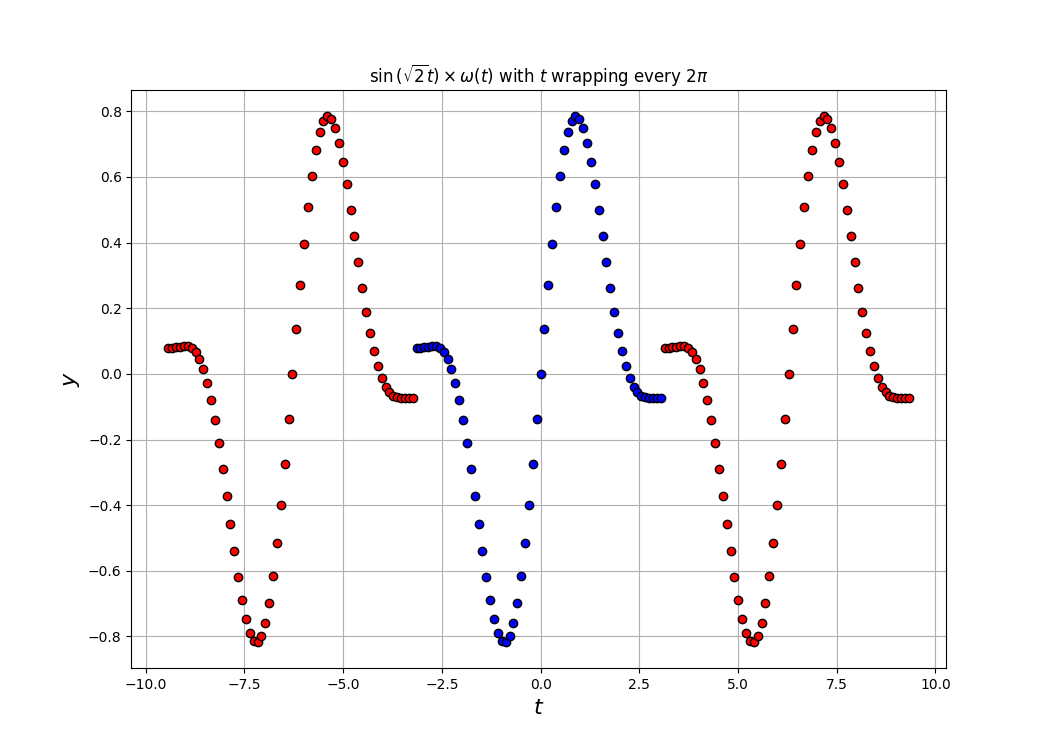
\includegraphics[height=11cm]{Figure_5.png}
\label{fig:exemplo}
\end{figure}

\newpage
\section*{Response of Damped sinusoidal with input of $2 \times 10^{5}$ Hz in HPF:}

Here is the Input and Output voltage plots for Damped sinusoidal inputs with $2 \times 10^{5}$ Hz frequency. We can notice that the input voltage's amplitude is not damping much.\\
\\While the Output voltage is sinusoidal, and it's amplitude increases slightly in beginning and maintains almost same amplitude thereafter.

\begin{figure}[h!]
\centering
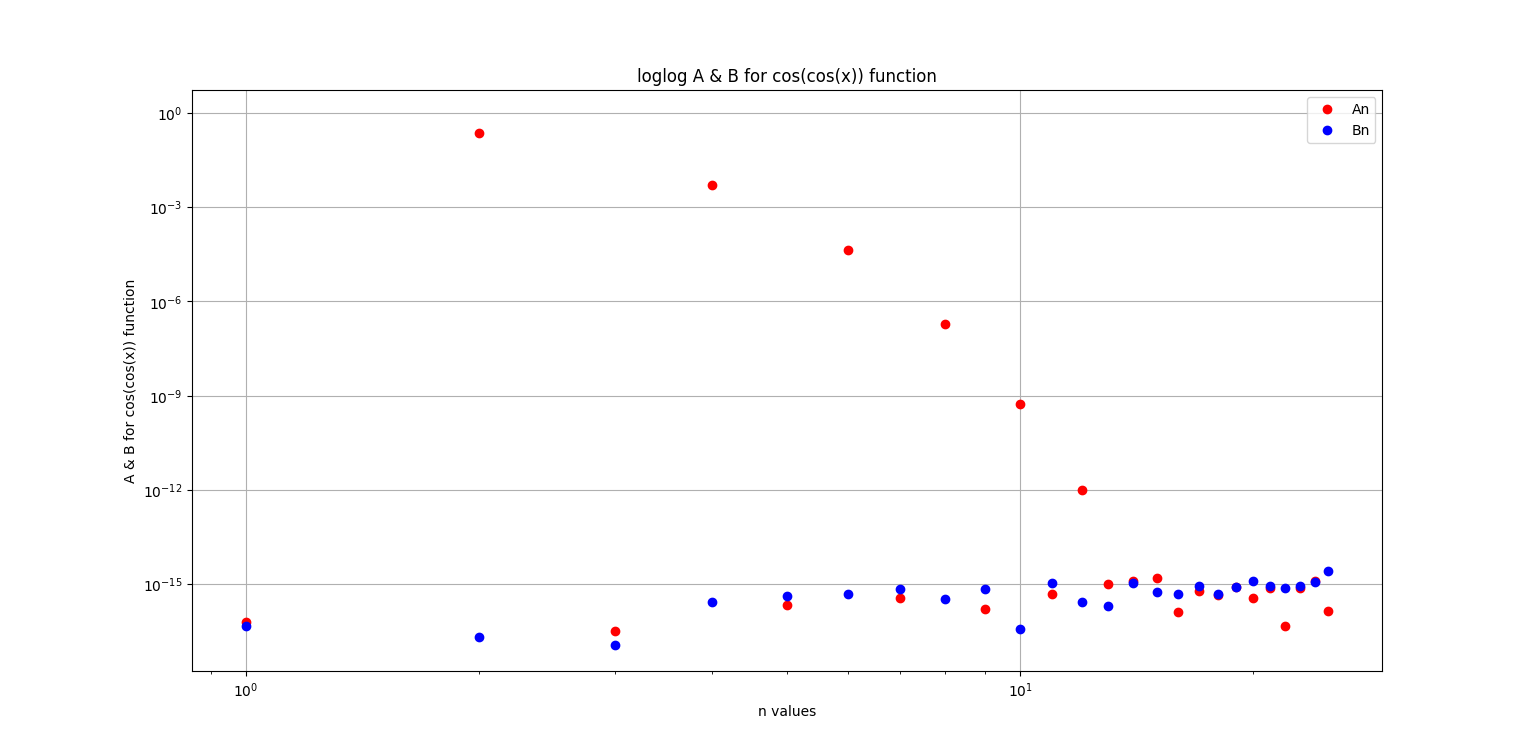
\includegraphics[height=10cm]{Figure_6.png}
\label{fig:exemplo}
\end{figure}

These above two plots clearly say the working principle of HPF. Thus, confirming that this is a HBF.

\newpage
\section*{Step response of the High pass filter:}

Step response of HPF is obtained from 'step' function from scipy.signal,\\\\
Here we can notice that the Output voltage is high at start, and then suddenly decreases drastically and increases a little and remains constant over rest of the time.

\begin{figure}[h!]
\centering
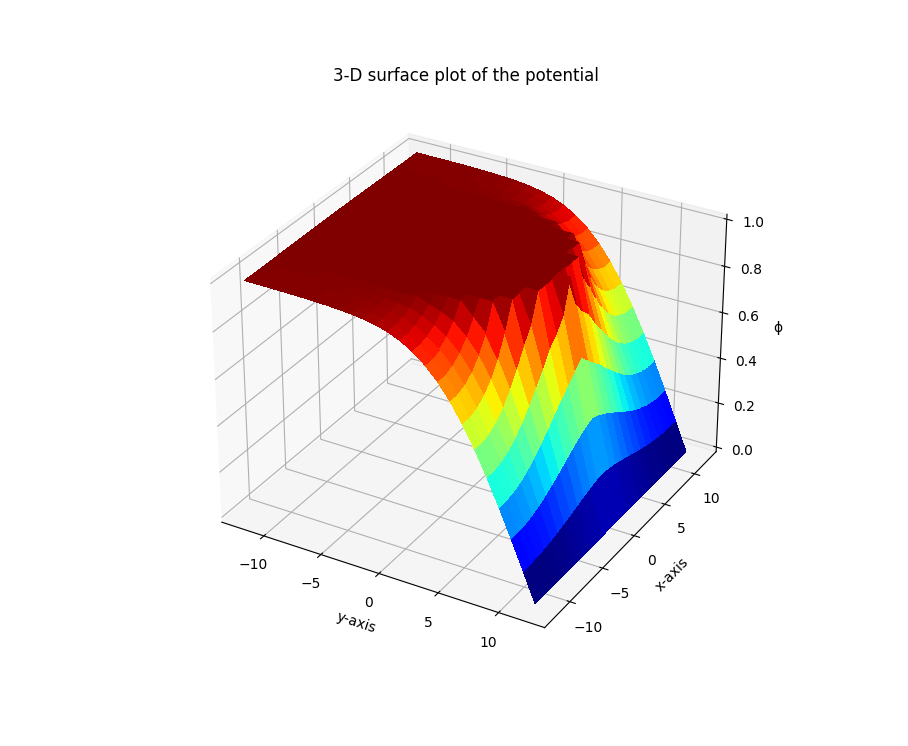
\includegraphics[height=12cm]{Figure_7.png}
\label{fig:exemplo}
\end{figure}

\section*{\textbf{Conclusion:}}
The functions like $'step'$ , $'lsim'$ , $'as\_numer\_denom'$ , $'lambdify'$ were very useful while working with tranfer functions. Thus, making solving of circuits and filters easy in python.

\begin{center} 
\textbf{Thank you!}
\end{center} 
\end{document}
